\section{theory}
\label{sec:theory}
The aim of this experiment is to record the absoption spectrum
of rubidium. Therefor a diode laser is adjusted and aimed towards a cell
filled with rubidum.
The following part introduce the theory
important for the understanding of the experiment.

\subsection{Semiconductor}
\label{subsec:Semiconductor}

The diode laser is a result of the reseaching done on semiconductor.
So first a deeper comprehension of semiconductor theory is needed.
Hence the principle funcion of a simple p-n diode is described.
A p-n diode exist out of two semiconductor materials one
n-type and the other p-type.
In the p-type semiconductor is an excess of holes
and in the n-type semiconductor, an exess of electrons.
An excess of holes or electrons can be accomplisht by doping.
When n- and p-type are merged together,
electrons and holes diffuse in opposite side and recombine.
This process induce a elctricfield bettween the fixed doping atoms, which
counteracts the diffusion process.
If equilibrium between the two forces is accomplisht
a charge depletion zone is created
at the p-n junction.
The figure \ref{fig:equi} shows
a schematic p-n Diode in equilibrium.

\begin{figure}
\centering
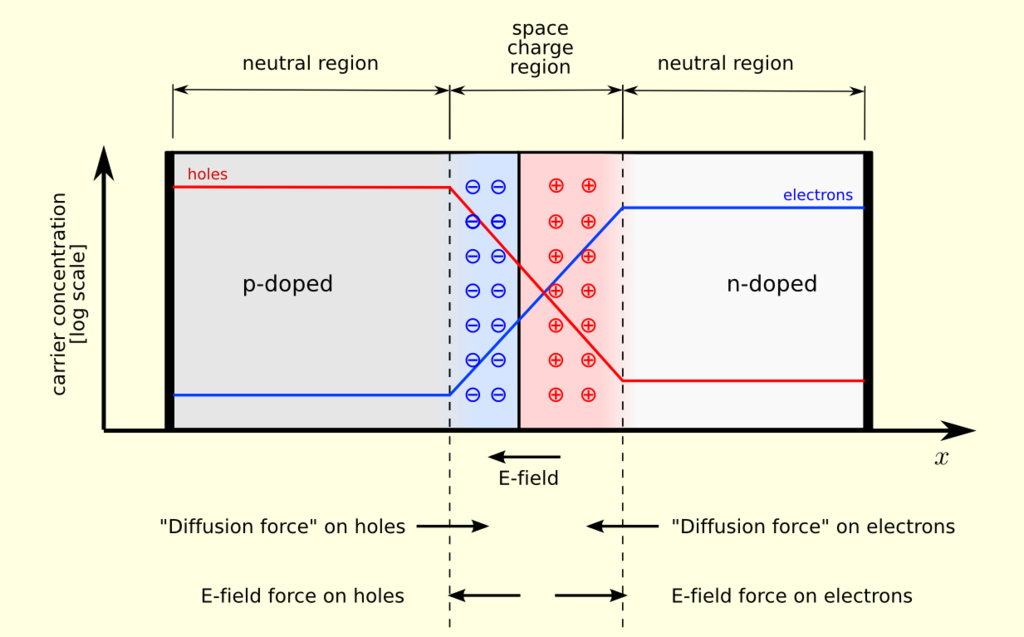
\includegraphics[width=0.7\textwidth]{equilibrium.png}
\caption{A schematic p-n Diode in equilibrium.
\cite{wiki_diode}}
\label{fig:equi}
\end{figure}
There are two possible ways apply voltage
in forward bias and
in rewerse bias.
In forward bias the diode let the curruent follow
but in the rewese bias the diode bocks the current. 



\begin{figure}
  \centering
  \includegraphics{plot.pdf}
  \caption{Plot.}
  \label{fig:plot}
\end{figure}


Because of this a diode has an





\subsection{Laser}
